\chapter{TINJAUAN PUSTAKA DAN KONSEP DASAR SISTEM}

\section{Desain Konsep Sistem}
\begin{figure}[h]
	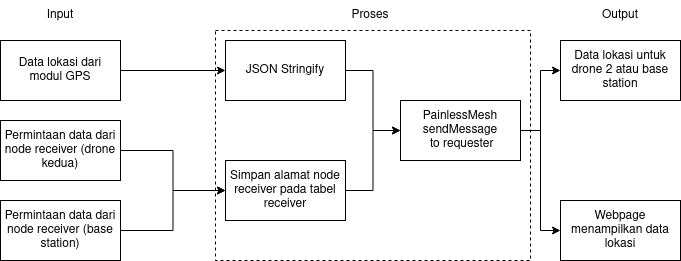
\includegraphics[scale=0.60]{./assets/IOProses}
	\caption{Desain konsep sistem}
\end{figure}
Gambar 2.1 menunjukkan desain konsep sistem secara dasar, dengan masukan sistem berupa data lokasi dari GPS dan permintaan data dari \textit{receiver}, proses data berupa pembuatan sebuah data JSON dari data lokasi GPS serta pengiriman data ke \textit{receiver}, dan keluaran berupa data lokasi yang diterima \textit{receiver}. Kemudian dari setiap data yang dikirimkan, akan dihitung besar \textit{throughput}, \textit{packet loss}, dan \textit{round-trip delay} jaringan serta mendapatkan besar \textit{signal strength} antar node jaringan.

\section{Riset Terkait}
Terdapat beberapa penelitian yang telah dilaksanakan sebelumnya yang terkait dengan tugas akhir ini, yang akan digunakan sebagai dasar atau referensi dalam pengerjaan. Beberapa penelitian terkait dapat dilihat pada tabel 2.1.
\pagebreak
\begin{center}
	\footnotesize
	\captionof{table}{Penelitian terkait}
	\begin{longtable}{|p{0.5cm}|p{2cm}|p{2cm}|p{2cm}|p{2cm}|p{2cm}|}
		\hline
		No.&\textbf{Judul}&\textbf{Metode}&\textbf{Kesimpulan}&\textbf{Kelebihan}&\textbf{Kekurangan}\\
		\hline
		\cite{santosUseHighMobility2021}&Use of High Mobility Nodes to Improve Connectivity in Wireless Sensor Networks&PainlessMesh-based Opportunistic Mobile Ad Hoc Networks&Menggunakan high mobility nodes berupa drone sebagai messenger data antara cluster sensor dengan server&Penelitian mengimplementasikan metode security berbasis secret-key cryptography. Packet loss antara sensor dan server rendah, hanya 4,48\% pada kondisi terburuk walaupun packet melewati 2 hop.
		&Tidak menguji round-trip delay packet\\
		\hline
		\cite{chiaPerformanceEvaluationESP82662019a}&Performance Evaluation of ESP8266 Mesh Networks&Pengujian one-way delay dan data rate pada jaringan PainlessMesh ESP8266& Jumlah node berkorelasi dengan meningkatnya single hop delay dan menurunnya stabilitas jaringan, serta besar payload menentukan data rate dan korupsi data.&Penelitian menguji dari 2 hingga 16 node sehingga terlihat gambaran kasar stabilitas jaringan PainlessMesh. Kinerja jaringan 2 node memiliki delay 2.49 ms sehingga cukup untuk aplikasi yang tidak terlalu kompleks.&ESP8266 tidak memiliki performa yang cukup untuk mengirimkan dan menerima payload data yang besar. Pengujian data rate dibatasi pada 2 node. \\
		\hline
		\cite{manviImplementingWirelessMesh2020}&Implementing Wireless Mesh Network Topology Between Multiple Wi-Fi Powered Nodes for IoT Systems&Penggunaan 3 node PainlessMesh berbasis ESP32 untuk komunikasi multidirectional output sensor dan input push button&Mesh bersifat self-healing, pada saat terjadi disrupsi maka mesh secara otomatis mengatur diri.&Implementasi 3 node dan arah data bolak balik dapat dilakukan&Tidak ada pengujian jarak jauh\\
		\hline
		\cite{guoDustSensorMonitoring2021}&A dust sensor monitoring system using Wi-Fi mesh network&Implementasi 9 node berbasis ESP32 dan ESP-Mesh untuk monitoring tingkat debu pada suatu ruangan.&Sistem efektif dengan measurement error dibawah 5\%&Mesh dapat berfungsi tanpa intervensi manusia, memiliki sifat self-healing dan auto-configuration.& Jaringan memiliki topologi tree, bukan mesh murni, sehingga jika terjadi gangguan pada node akar maka proses self-heal berjalan lebih lama.\\
		\hline
	\end{longtable}
\end{center}

Berdasarkan penelitian yang telah dilakukan sebelumnya, maka pada penelitian tugas akhir ini menggunakan 3 node jaringan, masing-masing berupa board mikrokontroler ESP32. 2 node ditempatkan pada UAV/drone quadcopter, dimana 1 node memiliki modul GPS sebagai pengirim data lokasi dan 1 node memiliki board MicroSD untuk \textit{data logging} serta sebagai penerima data lokasi dari pengirim. Node terakhir berada di darat dan berfungsi sebagai penerima data lokasi dari node pengirim serta menampilkan data tersebut kepada pengguna pada sebuah \textit{Web server}.

\section{\textit{Unmanned Aerial Vehicles} (UAV)}
\begin{figure}[H]
	\centering
	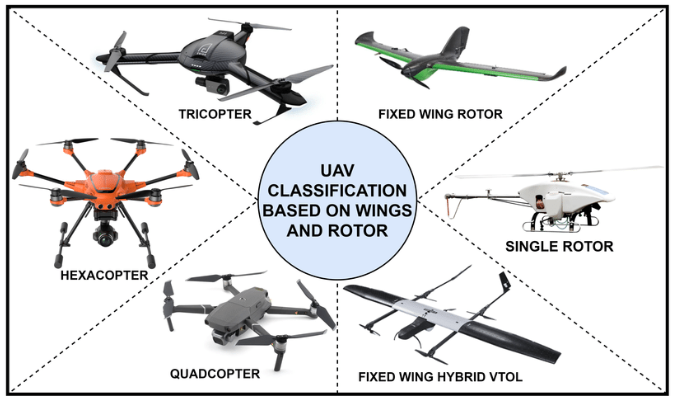
\includegraphics[scale=0.4]{./assets/TypesOfUAVs}
	\caption{Beberapa tipe-tipe UAV \cite{chamola_comprehensive_2020}}
\end{figure}
UAV adalah sebuah pesawat terbang yang dapat mengudara tanpa awak \cite{lakshminarayananJointNetworkDisaster2015}, dikendalikan secara \textit{remote} atau secara otonom. Salah satu tipe UAV adalah \textit{quadcopter drone}. Pada sistem ini, UAV digunakan sebagai pengirim data lokasi GPS sebagai node \textit{sender}, dan penerima data lokasi GPS sebagai node \textit{receiver}.

\section{\textit{Quadcopter}}
\begin{figure}[H]
	\centering
	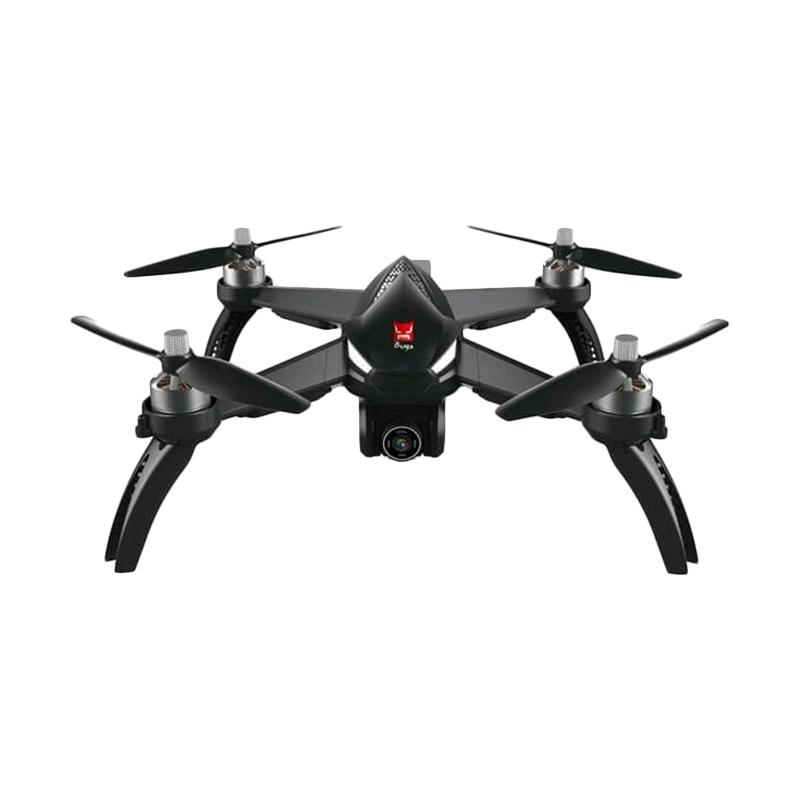
\includegraphics[scale=0.2]{./assets/MJX}
	\caption{Salah satu contoh \textit{quadcopter.}}
\end{figure}
Drone \textit{quadcopter} adalah suatu jenis UAV yang memiliki 4 rotor pada masing-masing sudut. Sama seperti helikopter, \textit{quadcopter} memiliki kemampuan untuk \textit{hover}. Terdapat sepasang rotor yang berputar searah jarum jam dan sepasang rotor yang berputar berlawanan arah jarum jam, sehingga pada kondisi \textit{steady state} total torsi pada \textit{drone} adalah nol. Hal tersebut juga menyebabkan konfigurasi \textit{quadcopter} tidak membutuhkan \textit{tail rotor}. Keempat rotor tersebut juga menghasilkan daya angkat yang besar, sehingga cocok digunakan untuk membawa \textit{payload}. Pada penelitian ini, setiap drone membawa payload berupa board mikrokontroler yang membuat sebuah jaringan nirkabel bersifat ad-hoc.

\section{Jaringan Nirkabel}
\textit{Wireless Network} atau jaringan nirkabel adalah sebuah jaringan komputer yang menggunakan media nirkabel untuk koneksi data antar node \cite{designing_a_wireless_network}. Melalui media nirkabel, sebuah jaringan bersifat lebih fleksibel dalam sebuah ruangan karena tidak terbatasi oleh perkabelan untuk berkomunikasi. Jaringan nirkabel dapat dikelompokkan berdasarkan besar lingkupnya:
\subsection{\textit{Wireless Wide Area Network} (WWAN)}
Sebuah \textit{Wide Area Network} (WAN) adalah jaringan dengan lingkup besar, yakni melingkupi sebuah daerah regional, negara, dan seluruh dunia \cite{data_communications_and_networking}. Sebuah jaringan nirkabel yang melingkupi sebuah WAN memerlukan teknologi yang dapat melayani node yang bergerak-gerak. Contoh dari teknologi WWAN adalah jaringan seluler dan \textit{wireless ad-hoc networks} (WANET).
\subsection{\textit{Wireless Local Area Network} (WLAN)}
\textit{Local Area Network} (LAN) adalah sebuah jaringan dengan lingkup lokal, seperti sebuah gedung/bangunan, atau sebuah daerah kecil seperti sebuah kampus. Sebuah jaringan WLAN dapat melayani pengguna yang bergerak dalam jaringan itu sendiri. Contoh dari teknologi WLAN adalah Wi-Fi (IEEE 802.11).
\subsection{\textit{Wireless Personal Area Network} (WPAN)}
\textit{Personal Area Network} adalah sebuah jaringan dengan lingkup pribadi dan biasa digunakan untuk komunikasi antar-piranti jarak pendek. Contoh dari teknologi WPAN adalah Bluetooth.

\section{\textit{Flying Ad-hoc Network}}
Menurut Khan (2017)  \cite{khanFlyingAdhocNetworks2017}, \textit{Flying Ad-hoc Network} adalah sebuah kumpulan UAV-UAV kecil dalam konfigurasi ad-hoc, mengadopsi model jaringan WANET. Terdapat beberapa pertimbangan dalam pemilihan jenis teknologi komunikasi nirkabel untuk sebuah jaringan FANET, yakni kemampuan untuk \textit{autoconfiguration}, tidak membutuhkan infrastruktur yang sudah ada, serta lingkup jaringan yang luas.
\subsection{Bluetooth untuk penggunaan FANET}
Terdapat dua jenis teknologi Bluetooth yang dipasarkan oleh Bluetooth SIG, yakni Classic Bluetooth dan Bluetooth Low Energy (LE). Masing-masing memiliki \textit{range} teoritis sebesar 100 meter, tetapi dengan batasan daya radio dan interferensi maka \textit{range} secara praktis hanya sekitar 10 sampai 20 meter \cite{noauthor_all_nodate}. Dengan target jarak antar node hingga 100 meter, maka teknologi Bluetooth kurang cocok untuk digunakan untuk FANET.
\subsection{Jaringan Seluler untuk penggunaan FANET}
Sebuah jaringan seluler membutuhkan infrastruktur penunjang untuk membangun jaringan tersebut, seperti \textit{Base Transceiver Station}, \textit{Base Station Controller}, dan \textit{Mobile Switching Center} \cite{noauthor_cellular_nodate}; sehingga teknologi jaringan seluler kurang cocok untuk digunakan pada aplikasi FANET penelitian ini karena tidak dapat berfungsi tanpa infrastruktur yang sudah ada.
\subsection{Wi-Fi untuk penggunaan FANET}
Implementasi protokol IEEE 802.11 tidak menentukan \textit{range} maksimum dari jaringan Wi-Fi, sehingga \textit{range} maksimum dapat bervariasi sangat drastis. Dengan mengubah implementasi IEEE 802.11 pada sebuah piranti, maka jarak antar piranti dapat ditingkatkan dengan mengorbankan kemampuan interoperabilitas dengan piranti Wi-Fi lain. Contohnya adalah implementasi Espressif 802.11 Long Range, yang mengklaim dapat memiliki jarak maksimum hingga 1 km dengan \textit{line-of-sight} \cite{noauthor_wi-fi_nodate}. 

Wi-Fi juga dapat berfungsi tanpa adanya infrastruktur yang sudah ada menggunakan mode ad-hoc, sehingga piranti berbasis Wi-Fi dapat berkomunikasi satu sama lain tanpa memerlukan sebuah titik sentral seperti Wi-Fi router. Sehingga Wi-Fi cocok digunakan untuk jaringan FANET pada tugas akhir ini.

\section{Jaringan \textit{mesh}}
Jaringan \textit{mesh} adalah sebuah topologi jaringan dimana masing-masing node jaringan terhubung satu sama lain secara non-hierarkis. Pada sebuah jaringan \textit{mesh} penuh, setiap node memiliki sebuah \textit{routing} terhadap satu sama lain, sedangkan pada jaringan \textit{mesh} parsial, hanya beberapa titik node yang terhubung satu sama lain, sehingga pada beberapa kasus data perlu melewati node lain untuk menuju node tujuan.

\begin{figure}[h]
	\centering
	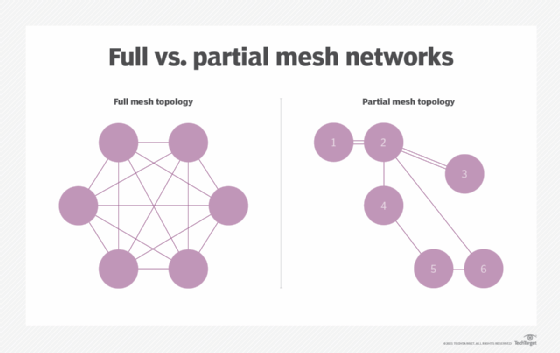
\includegraphics[scale=0.5]{./assets/meshpartial}
	\caption{Bentuk topologi jaringan \textit{mesh} penuh dan parsial}
\end{figure}

\section{ESP32}
ESP32 adalah sebuah mikrokontroler \textit{system-on-a-chip} dengan integrasi Wi-Fi dan Bluetooth dan biaya yang murah. Dengan modul dibuat oleh Espressif Systems, ESP32 dapat digunakan dalam bentuk chip sendiri, atau menggunakan \textit{development board} buatan produsen lain.

Terdapat beberapa variasi modul ESP32, dengan versi CPU \textit{single core} berbasis RISC-V dan \textit{dual core} berbasis Xtensa LX7. Setiap modul ESP32 mendukung protokol Wi-Fi 802.11b/g/n pada band 2.4 GHz. ESP32 mendukung mode operasi klien Wi-Fi \textit{(station mode)}, mode operasi \textit{Access Point} Wi-Fi, dan mode keduanya sekaligus (APSTA). Fitur ini dapat digunakan untuk membuat sebuah jaringan \textit{mesh} ad-hoc.

ESP32 juga mendukung protokol \textit{proprietary} buatan Espressif bernama 802.11 LR \textit{(Long Range)}, dengan jarak hingga 1 km selama ada \textit{line-of-sight} antara \textit{node}. \cite{WiFiDriverESP32}.
\begin{figure}[h]
	\centering
	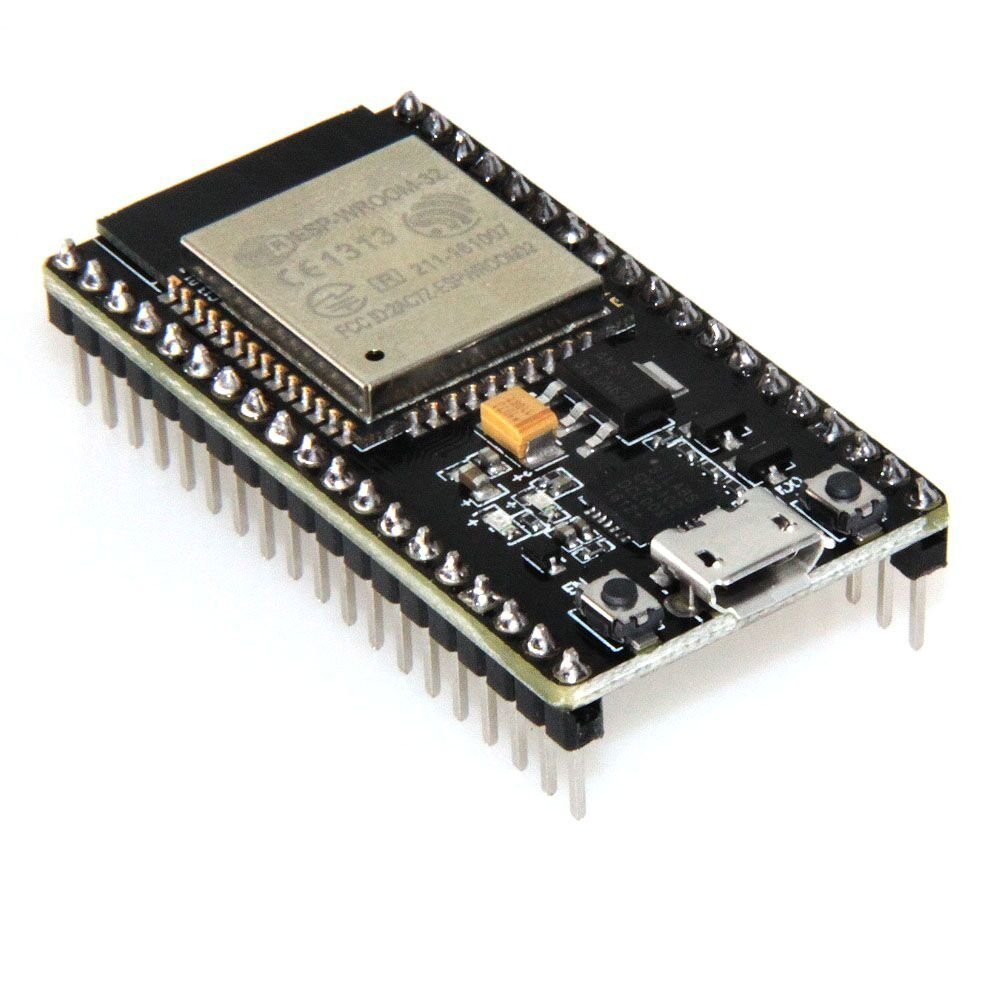
\includegraphics[scale=0.1]{./assets/ESP32}
	\caption{ESP32}
\end{figure}

\section{PainlessMesh}
PainlessMesh merupakan sebuah library yang memudahkan pengguna \textit{board} ESP32 dalam membuat sebuah jaringan mesh ad-hoc berbasis WiFi. Karena batasan dari \textit{board} ESP32, maka jaringan yang dihasilkan merupakan \textit{partial mesh} sehingga pada kondisi standar, semua node memiliki kedudukan yang sama dan diatur dalam topologi campuran antara \textit{tree} dengan \textit{mesh}.

Jaringan PainlessMesh menggunakan mode APSTA pada board ESP32, dimana setiap board ESP32, disebut dengan "node", berfungsi sebagai WiFi \textit{Access Point} (AP) sekaligus sebagai klien WiFi \textit{Station Mode}. Setiap node berbasis ESP32 dapat memiliki sebanyak 10 klien yang terhubung pada 1 AP, dan dapat terhubung pada AP lainnya sebagai sebuah klien.

\begin{figure}[h]
	\centering
	\includegraphics[scale=0.5]{./assets/painlessmesh}
	\caption{Topologi jaringan PainlessMesh \cite{HomeWikiPainlessMesh}, panah menunjukkan arah koneksi dari klien ke AP}
\end{figure}

Keistimewaan dari library PainlessMesh adalah kemampuannya untuk \textit{autoconfigure}, dimana setiap node dapat memutus sambungan dan menyambung ulang setiap saat, dan jaringan mesh dapat berjalan melalui proses konfigurasi secara otomatis.

\subsection{Protokol PainlessMesh}
Setiap pesan yang dikirimkan dalam sebuah jaringan PainlessMesh adalah berbasis JavaScript Object Notation (JSON), dan dapat dibagi menjadi dua tipe pesan: \textit{control messages} dan \textit{user messages}.

\textit{Control messages} adalah pesan yang dikirimkan secara otomatis oleh \textit{library} PainlessMesh untuk menjaga kelangsungan jaringan mesh secara asinkron, seperti sinkronisasi waktu antar node dan informasi \textit{routing} antar node. \textit{Control messages} hanya dikirimkan antara node yang berhubungan langsung satu sama lain.

\textit{User messages} adalah pesan yang dikirimkan oleh pengguna dalam jaringan PainlessMesh, dan dapat berupa \textit{string}, \textit{binary data}, dan data JSON yang disematkan dalam \textit{user message} tersebut. Setiap \textit{user message} dapat ditentukan tujuannya antara tujuan spesifik (\textit{single addressed}) maupun \textit{broadcast}.

\subsection{JavaScript Object Notation (JSON)}
PainlessMesh menggunakan JavaScript Object Notation untuk setiap pengiriman pesan antar-node dalam jaringan. Penggunaan JSON memudahkan penafsiran \textit{(parsing)} setiap pesan yang diterima untuk kemudian diolah menjadi data yang ditampilkan \cite{MeshProtocolWiki}.

\begin{figure}[h]
	\centering
	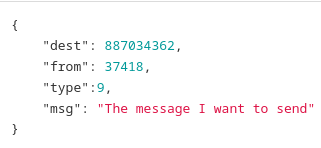
\includegraphics[scale=0.5]{./assets/PainlessMeshJSON}
	\caption{Setiap pesan pada jaringan PainlessMesh menggunakan JSON.}
\end{figure}

Setiap paket data PainlessMesh menggunakan skema JSON untuk menentukan tujuan (dari \textit{key "dest"}), dari mana paket data tersebut berasal (\textit{key "from"}), jenis paket berdasarkan nilai integer pada \textit{key "type"}, serta pesan yang akan dikirim pada \textit{key "msg"}.

\section{\textit{Global Positioning System} (GPS)}
GPS adalah sebuah sistem navigasi satelit yang dikembangkan oleh United States Department of Defense (US DoD) dan dimiliki oleh pemerintah Amerika Serikat. Dengan menggunakan data waktu atomik dan beberapa satelit, maka lokasi (lintang, bujur, dan ketinggian) sebuah \textit{receiver} GPS dapat didapatkan dengan akurasi sisi satelit yang dijamin oleh pemerintah Amerika Serikat kurang dari 2 meter \cite{noauthor_gpsgov_nodate}.

Data lokasi dapat diterima dari satelit GPS menggunakan GPS \textit{receiver}. Pada beberapa \textit{receiver} GPS, data yang diterima adalah berupa data National Marine Electronics Association (NMEA) 0183.

\section{GPS NMEA Data}
Modul GPS NEO-6M menghasilkan output serial mentah berupa data NMEA 0183, sebuah standar komunikasi piranti GPS berupa karakter-karakter ASCII yang membentuk kalimat-kalimat NMEA \cite{GPSNMEASentence}.

\begin{figure}[H]
	\centering
	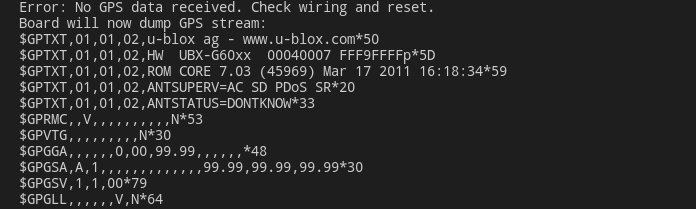
\includegraphics[scale=0.5]{./assets/NMEASentences}
	\caption{Contoh data mentah dari modul GPS NEO-6M berupa data GPS NMEA.}
\end{figure}

\section{Pengukuran Kinerja Jaringan}
\subsection{Round-trip delay}
\textit{Round-trip delay} adalah waktu yang diperlukan untuk sebuah paket data dikirimkan dari node pengirim ke node penerima, ditambah waktu yang diperlukan untuk paket \textit{acknowledge} diterima oleh node pengirim dari node penerima. Pengukuran \textit{round-trip delay} dapat menggunakan fungsi yang sudah diimplementasikan dalam \textit{library} PainlessMesh yakni \verb|painlessMesh::startDelayMeas()|.

Setiap node pada jaringan PainlessMesh memiliki waktu internal yang tersinkronisasi satu sama lain melalui proses \textit{"Time sync"} \cite{MeshProtocolWiki} yang berlangsung secara periodis setiap 10 menit. PainlessMesh menjaga waktu jaringan pada tingkat kepresisian mikrosekon menggunakan fungsi \verb|micros()| pada mikrokontroler ESP32. Kemudian setelah fungsi \verb|startDelayMeas()| dipanggil, maka \textit{round-trip delay} dapat dihitung menggunakan rumus berikut:

\begin{equation}
	 t_{round trip} = (t_3 - t_0) - (t_2 - t_1)
\end{equation}

$t_0$ = waktu internal pada pengirim \textit{delay measurement}\\
$t_1$ = \textit{timestamp} pada saat paket \textit{delay measurement} diterima\\
$t_2$ = \textit{timestamp} pada saat respon terhadap \textit{delay measurement} dikirimkan\\
$t_3$ = \textit{timestamp} pada saat respon diterima oleh pengirim \textit{delay measurement}

\subsection{Throughput}
\textit{Throughput} adalah banyaknya data yang dapat ditransmisikan dalam suatu satuan waktu. Pada penelitian ini, \textit{throughput} dihitung setiap pengiriman paket data, dibandingkan dengan perbedaan \textit{timestamp} antara pengiriman dan penerimaan paket data tersebut.

\begin{equation}
	Throughput = \frac{sizeof(packet)}{t_1 - t_0}
\end{equation}
$t_0$ = waktu internal pada saat pengirim mengirim paket data\\
$t_1$ = \textit{timestamp} pada saat penerima menerima paket data

\subsection{Packet loss}
Packet loss adalah jumlah packet data yang hilang dibandingkan packet data yang berhasil dikirimkan.
\begin{equation}
	Packet Loss = (1 - \frac{ack_{RX}}{p_{TX}})\times 100\%
\end{equation}

$p_{TX}$ = jumlah packet data yang dikirimkan\\
$ack_{RX}$ = jumlah packet respon yang diterima

\begin{figure}[H]
	\centering
	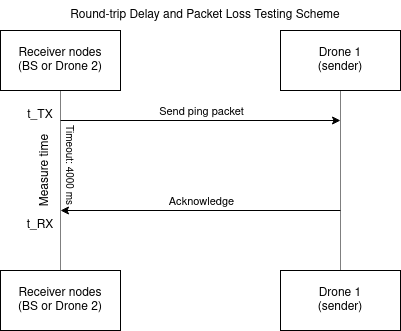
\includegraphics[scale=0.7]{./assets/PingTest}
	\caption{Skema pengujian \textit{round-trip delay} dan \textit{packet loss}}
\end{figure}